\documentclass[11pt]{jsarticle}

\usepackage{SPR}

\headerSPR
\begin{document}
	\titleSPR{\number\year}{\number\month}{\number\day}{D2}{吉田 皓太郎}
%%%%%%%%%%%%%%%%%%%%%%%%%%%%%%%%%%%%%%
	\articleSPRabst
		\begin{itemize}
			\item 機械学習を用いたカップ形状の設計支援
			\item 着後形状予測のためのカップの変形解析
		\end{itemize}
		
		
	\articleSPRobj
		\begin{enumerate}
			\item 定性的な機能要求を満たせるようなカップ形状を設計できる
			\item 布の物性とカップのパターンがどのような結びつきを持っているかを調べることができる.
		\end{enumerate}
%%%%%%%%%%%%%%%%%%%%%%%%%%%%%%%%%%%%%%
% 1.前回からのノルマ
	\articleSPRitemsone
		%\begin{enumerate}
		%	\item A
		%\end{enumerate}
		
		\tableofcontents
		
		
%%%%%%%%%%%%%%%%%%%%%%%%%%%%%%%%%%%%%%
%\begin{itemize}
%	\item 新規手法について
%	\item ISFAアウトライン
%\end{itemize}
%%%%%%%%%%%%%%%%%%%%%%%%%%%%%%%%%%%%%%
% 2.具体的な成果
	\articleSPRitemstwo
	\renewcommand{\labelitemi}{$\blacktriangledown$}
	%\renewcommand{\labelitemi}{$\bigcirc$}
	\newcommand{\argmax}{\mathop{\rm arg~max}\limits}
	\newcommand{\argmin}{\mathop{\rm arg~min}\limits}
	\newcommand{\Ker}{{\rm Ker}}
	\newcommand{\rank}{{\rm rank}}
%%%%%%%%%%%%%%%%%%%%%%%%%%%%%%%%%%%%%
	\section{研究進捗について}
		\subsection{システムの概要}
			本研究で示すシステムは,設計工学会で発表したシステムを応用し,ある目的の出力値に対してそれを満たす形状を復元するシステムについて考える.前提として,出力を行う機械学習モデルはすでに出来上がっていると想定する.この時,形状得るまでの過程をフローにまとめると以下のように表される.
			\begin{figure}[!h]
				\centering
				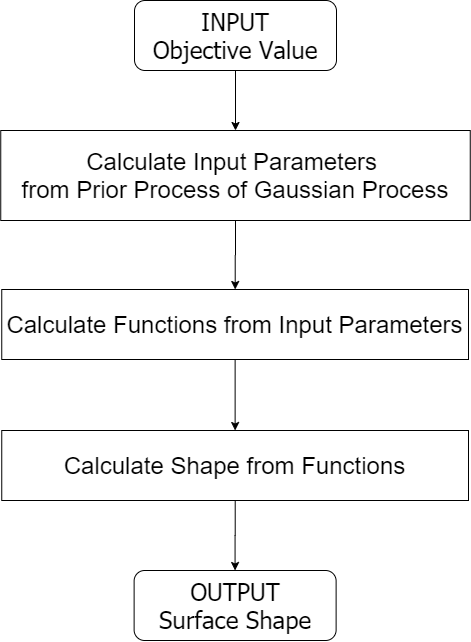
\includegraphics[width = 0.3\columnwidth]{./figure/flowoutput.png}
				\caption{flow chart}
			\end{figure}
			最初のステップは,事後学習式$ \mu(\bd{x}_*) = \{ k_i (\bd{x}_*)\}^T (\bd{K} + \sigma^2 \bd{I})^{-1} \bd{y} $を求根アルゴリズムを適用することによって,得られると考えられる.今回はそれによってパラメータが得られた時,そのパラメータから形状を復元させる手法を考える.
			
			求めたい可展面形状は,その曲面上に存在する2つの曲線によって決定される.今回は下ワイヤーが与えられていることから,対応する上下接ぎラインを得ることを目標とする.この上下接ぎラインを決定するためには,曲線形状を決定する物体標講の回転率ベクトル$ \bd{\omega} $の他に,2つの曲線の弧長間の対応$ u=u(s) $を決定する必要がある.この上下接ぎラインを求める問題は,下記の可展面条件を最小化するという最適化問題として定式化される.
			\begin{equation}\label{eq:DevCond_eq}
					\mathrm{find}\; \bd{\omega},u(s) \;\; \mathrm{s.t.} \; \min \int_{0}^{L} |(\bd{\zeta}_L \times \bd{\zeta}_U) \cdot (\bd{x}_U - \bd{x}_L)| ds					
			\end{equation}
			上下接ぎラインの情報を用いて,$ \alpha,\omega_{\eta},D $に関しては,それぞれ次式で表される.
			\begin{eqnarray}
			D &=& |\bd{x}_U - \bd{x}_L|\\
			\alpha &=& -\sin^{-1} \bd{g} \cdot \bd{\zeta}_L\\
			\omega_{\eta} &=& \frac{\bd{g} \cdot \bd{\zeta}_L'}{\cos \alpha}
			\end{eqnarray}
			ただし,$ \bd{g}  = \frac{\bd{x}_U - \bd{x}_L}{D}$である.パラメータに関する条件から,$ \alpha,\omega_{\eta},D  $に関しては,次式で示す対数尤度に関する条件を満たす必要がある.
			\begin{equation}\label{eq:st.likelihood}
				\max -\log|\bd{K}_i| - \bd{y}_i^T \bd{K}_{\theta_i}^{-1} \bd{y}_i \;\; i\in [\alpha,\;\omega_{\eta},\;D]
			\end{equation}
			この問題は目的関数が複数ある多目的最適化問題として考えることができるが,計算コストの面では非効率的であると思われる.そこで,この問題を単一な目的関数の最適化問題に置き換えることを考える.
			
			\req{eq:st.likelihood}を,$ \bd{y} $に関する最適化問題として捉えるとき,この問題は二次形式$ \bd{y}_i^T \bd{K}_{\theta_i}^{-1} \bd{y}_i $の最小化問題へ置き換えることができる.グラム行列$ \bd{K}_{\theta_i}^{-1} $は正定値性が保証されているが,パラメータの与え方によっては隣接する行ベクトル同士の差分が小さくなり,行列が悪条件(逆行列の数値計算誤差が大きくなる)場合がある.このような場合は,できる限り逆行列を直接計算することを避ける必要がある.そこで,$ \bd{y} = \bd{K}\bd{a} $を満たす$ \bd{a} $を仮定し,\req{eq:st.likelihood}を書き直すと次式で表現される.
			\begin{equation}\label{eq:st.likelihood2}
				\bd{y}_i^T \bd{K}_{\theta_i}^{-1} \bd{y}_i  = \bd{a}_i^T \bd{K}_{\theta_i} \bd{a}_i \;\; i\in [\alpha,\;\omega_{\eta},\;D]
			\end{equation}
			ある二次形式$ \bd{x}^T \bd{A} \bd{x} $は,$ \bd{x}\cdot \bd{x} = 1 $の条件下で,その最大値・最小値は$ \bd{A} $の固有値と等しくなる.つまり,\req{eq:st.likelihood}で表される条件は,以下のような制約に変換可能である.
			\begin{equation}\label{eq:likelihoodCond}
				 \frac{\bd{a}_i^T \bd{K}_{\theta_i} \bd{a}_i }{\bd{a} \cdot \bd{a}} - \lambda_{\min}
			\end{equation}
			実際のプログラムでは,$ \lambda_{\min} $の値が他の制約に比べて小さいことから,以下のように相対的な誤差として制約を置いた.
			\begin{equation}\label{eq:likelihood_cond_by_program}
				\frac{\bd{a}_i^T \bd{K}_{\theta_i} \bd{a}_i }{\bd{a} \cdot \bd{a} \lambda_{\min}} -1 
			\end{equation}
			このパラメータに関する制約は,言い換えると曲面の内在的な性質にのみ着目し制約をかけていることに等しい.すなわち,可展面を求める問題に対し平面という局所解を許容している.このような局所解に陥らないように,目的関数に以下のようなバリア関数を加えた.今回の$ \lambda $は,0.1に設定している.
			\begin{equation}
				\lambda \int_{0}^{L} \frac{1}{(\kappa - |\omega_{\eta}|)^2} ds
			\end{equation}
			
			計算結果を示す.制約に関しては二次形式に関する制約がだいたい数$ \% $程度の誤差にはなったところを終了判定の基準定めた.
			形状の比較をすると,zy平面からの形状はとても近しいが,zx平面で確認する図では,似てはいるが少し異なった形を出力した.
			
			しかし,対応する出力値$ \phi_1 \frac{V}{S} $を比較すると,だいたい相対誤差は非常に近く$ 1.0\times 10^{-7} \% $ほどとなった.この結果から,完全に元の形には復元できるとは限らないが,その目的の値に合わせた曲面形状を導出することができたと結論づけることはできる.
			
			
			
			得られた結果とパラメータ元の形状比較
			\begin{figure}
				\begin{minipage}{0.5\hsize}
					\centering
					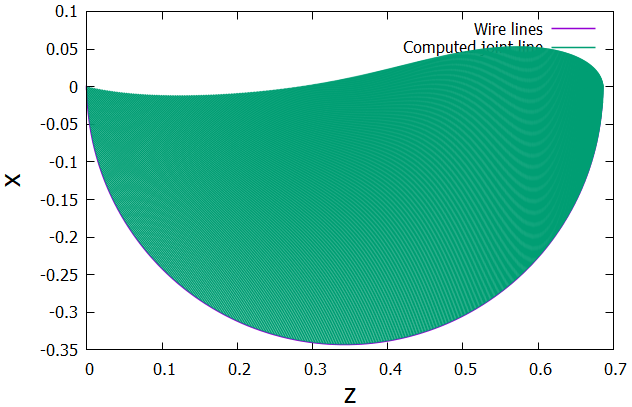
\includegraphics[width = \columnwidth]{./figure/ObtainedRidgeLinefromz-x.png}
				\end{minipage}
				\begin{minipage}{0.5\hsize}
					\centering
					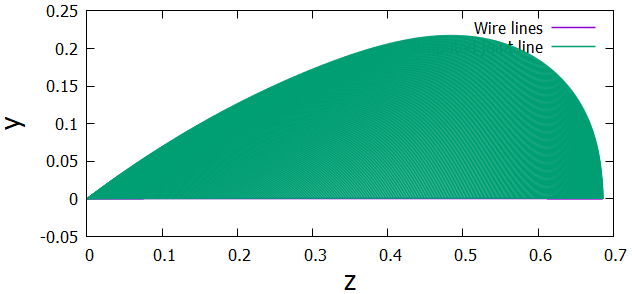
\includegraphics[width = \columnwidth]{./figure/ObtainedRidgeLinefromz-y.png}
				\end{minipage}
				\caption{元データ}
			\end{figure}
			\begin{figure}
				\begin{minipage}{0.5\hsize}
					\centering
					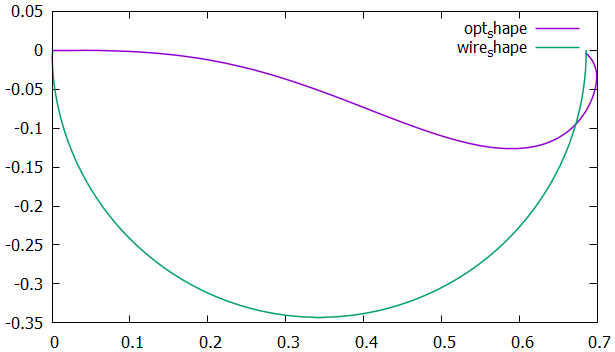
\includegraphics[width = \columnwidth]{./figure/0129/AlignWire_xyview.png}
				\end{minipage}
				\begin{minipage}{0.5\hsize}
					\centering
					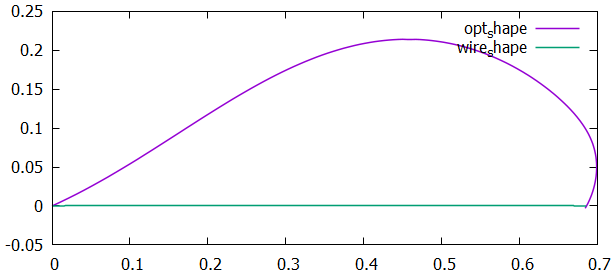
\includegraphics[width = \columnwidth]{./figure/0129/AlignWire_xzview.png}
				\end{minipage}
			\caption{得られた形状}
			\end{figure}
		
		\subsection{ISCIEネタ再投稿の件について}
			緒論をとりあえず日本語で書きました.
	\section{To Do List}
		\begin{itemize}
			\item 投稿論文修正・文章再考
			\item 投稿論文のためのスクリプト作成し,追加数値実験を行う
		\end{itemize}
				
	\newpage
\vspace{10cm}
%%%%%%%%%%%%%%%%%%%%%%%%%%%%%%%%%%%%%%
% 3.達成できなかったこととその問題点
	%\articleSPRthree
	
%%%%%%%%%%%%%%%%%%%%%%%%%%%%%%%%%%%%%%

\vspace{14cm}
%%%%%%%%%%%%%%%%%%%%%%%%%%%%%%%%%%%%%%
	\articleSPRfour
	\articleSPRfive
\end{document}
